Supongamos que tenemos una cadena $x$ de longitud $n$ y una cadena $y$ de longitud $m$, y queremos calcular la distancia de edición entre $x$ e $y$.

Para resolver el problema utilizando programación dinámica es necesario
plantearlo como una sucesión de decisiones que satisfaga el principio de óptimo.
Para plantearla, vamos a fijarnos en el último elemento de cada una de las
cadenas. Si los dos son iguales, entonces tendremos que calcular el número de
operaciones básicas necesarias para obtener de la primera cadena menos el último
elemento, y la segunda cadena también sin el último elemento, es decir:

$$ distance(n,m) = distance(n-1,m-1) \quad \text{si} \quad x_n = y_m$$ 

Pero si los últimos elementos fueran distintos habría que escoger la situación
más beneficiosa de entre tres posibles: (i) considerar la primera cadena y la
segunda pero sin el último elemento, o bien (ii) la primera cadena menos el último
elemento y la segunda cadena, o bien (iii) las dos cadenas sin el último elemento.
Esto da lugar a la siguiente relación en recurrencia para $distance(n,m)$ para este caso:

$ distance(n,m) = 1 + \min \{ distance(n-1,m), distance(n,m-1),distance(n-1,m-1) \} \quad \text{si} \quad n\neq  0, m \neq  0, x_n \neq y_m $

En cuanto a las condiciones iniciales, tenemos las tres siguientes:

$$distance(0,0)=0, \qquad  distance(n,0)=n, \qquad distance(0,m)=m,$$

Una vez disponemos de la ecuación en recurrencia necesitamos resolverla
utilizando alguna estructura que nos permita reutilizar resultados intermedios.

Para resolver el problema, definimos una función $distance(a,b)$ que proporciona la distancia de edición entre prefijos $x[0 \dots a]$ y $y[0 \dots b]$. Por lo tanto, al usar esta función, la distancia de edición entre $x$ e $y$ es igual a la distancia ($n-1$,$m-1$).

Podemos calcular los valores de distancia de la siguiente manera:
$$
\begin{array}{cl}
distance ( a, b ) =	& min( distance ( a, b-1) + 1,  \\
	& distance ( a - 1, b ) + 1, \\
	& distance ( a - 1, b - 1) + cost ( a, b ))
\end{array}
$$



Aquí $cost( a, b ) = 0$ si $x[a]=y[b]$, y en caso contrario $cost(a,b)=1$. La fórmula considera las siguientes formas de editar la cadena $x$:

\begin{itemize}
	\item distance($a, b-1$): inserta un carácter al final de $x$.
    \item distance($a-1, b$): remueve el ultimo carácter de $x$.
    \item distance($a-1, b-1$): coincide o modifica el último carácter de $x$.
\end{itemize}

En los dos primeros casos, es necesaria una operación de edición (insertar o eliminar). En el último caso, si $x[a] = y[b]$, podemos hacer coincidir los últimos caracteres sin editar; de lo contrario, se necesita una operación de edición (modificar).

La siguiente tabla muestra los valores de distancia en el caso de ejemplo:

% TODO: \usepackage{graphicx} required
\begin{figure}[h!]
	\centering
	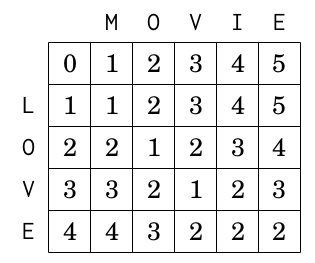
\includegraphics[width=0.3\linewidth]{img/edit_distance}
	\label{fig:editdistance}
\end{figure}


La esquina inferior derecha de la tabla nos dice que la distancia de edición entre LOVE y MOVIE es 2. La tabla también muestra cómo construir la secuencia más corta de operaciones de edición. En este caso el camino es el siguiente:

\begin{figure}[h!]
	\centering
	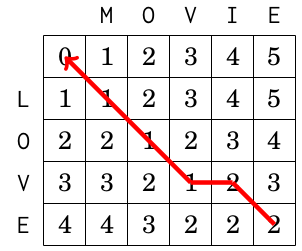
\includegraphics[width=0.3\linewidth]{img/edit_distance_2}
	\label{fig:editdistance2}
\end{figure}

Los últimos caracteres de LOVE y MOVIE son iguales, por lo que la distancia de edición entre ellos es igual a la distancia de edición entre LOV y MOVI. Podemos usar una operación de edición para eliminar el carácter I de MOVI. Por lo tanto, la distancia de edición es uno mayor que la distancia de edición entre LOV y MOV, etc.